\documentclass[11pt,a4paper]{article}
\usepackage[utf8]{inputenc}
\usepackage[spanish]{babel}
\usepackage{fullpage} % esto hace la página mas ancha, queda mejor? (SI!)
\usepackage{verbatimbox}
\usepackage{indentfirst}
\usepackage{graphicx}
\usepackage{courier}
\usepackage{float}

\begin{document}

\title{TP EDyA 1 - Cubo de Rubik}

\maketitle

\abstract{La idea de este trabajo es realizar un programa que resuelva un cubo de Rubik, de manera general, representando el problema como una búsqueda. El programa recibirá por su entrada estándar un cubo de Rubik y deberá imprimir por su salida estándar la secuencia de movimientos que lo resuelven (no necesariamente la secuencia óptima).}

\section{Introducción}

El cubo de Rubik es un rompecabezas mecánico tridimensional inventado por el escultor y profesor de arquitectura húngaro Ernö Rubik en 1974. Originalmente llamado ``cubo mágico'', el rompecabezas fue licenciado por Rubik para ser vendido por Ideal Toy Corp. en 1984 y ganó el premio alemán a mejor juego del año en la categoría ``Mejor Rompecabezas'' ese mismo año. Hasta enero de 2009 vendieron 350 millones de cubos en todo el mundo, haciéndolo el juego de rompecabezas más vendido del mundo. Es considerado ampliamente el juguete más vendido del mundo. \\

En un cubo de Rubik clásico, cada una de las seis caras está cubierta por nueve pegatinas de seis colores uniformes (tradicionalmente blanco, rojo, azul, naranja, verde y amarillo). Un mecanismo de ejes permite a cada cara girar independientemente, mezclando así los colores. Para resolver el rompecabezas, cada cara debe volver a consistir en un solo color.\\

El cubo de Rubik tiene ocho vértices y doce aristas. Hay $8!$ formas de combinar los vértices del cubo. Siete de estas pueden orientarse independientemente, y la orientación de la octava dependerá de las siete anteriores, dando  $3^7$ posibilidades. A su vez, hay $\frac{12!}{2}$ formas de disponer los vértices, dado que una paridad de las esquinas implica asimismo una paridad de las aristas. Once aristas pueden ser volteadas independientemente, y la rotación de la duodécima dependerá de las anteriores, dando $2^{11}$ posibilidades. En total el número de permutaciones posibles en el Cubo de Rubik es de:\\
\\
 $$ \frac{8!*12!*3^7*2^{11}}{2} = 43 \,.\, 252 \,.\, 003 \,.\, 274 \,.\, 489 \,.\, 856 \,.\, 000 $$ \\
 
Es decir, cuarenta y tres trillones doscientos cincuenta y dos mil tres billones doscientos setenta y cuatro mil cuatrocientos ochenta y nueve millones ochocientas cincuenta y seis mil permutaciones.\\

Recientemente (2008), se demostró que cualquier cubo puede ser resuelto en a lo sumo 20 movimientos \cite{movs}. No es necesario que el programa dé una solución óptima, cualquier receta\footnotemark  \, que lleve a resolver el cubo (de longitud razonable, digamos menor a 1000 movimientos) es válida.

\footnotetext{Se conoce como \emph{Receta} a cualquier secuencia de movimientos de las caras del cubo. Ejemplo: \texttt{RFlrUdbUU}}

\section{Comportamiento del programa}

\subsection{Entrada}
El cubo se representa en la entrada por su ``desdoblamiento''. El programa recibirá una cadena de 54 números representando al cubo, donde los números del 1 al 6 representan un color del cubo. Por ejemplo, el siguiente es un cubo resuelto: \\
\begin{center}
\begin{verbbox}
      1 1 1 
      1 1 1 
      1 1 1 
2 2 2 3 3 3 4 4 4 5 5 5 
2 2 2 3 3 3 4 4 4 5 5 5 
2 2 2 3 3 3 4 4 4 5 5 5
      6 6 6 
      6 6 6 
      6 6 6 
\end{verbbox}

\theverbbox
\end{center}

No se debe confiar en el espaciado de la entrada. Sólo se debe asumir que se darán como entrada 54 números representando a los colores de las caras, en el orden anterior. Es decir, la entrada anterior es equivalente a:

\begin{center}
\begin{verbbox}
1 1 1 1 1 1 1 1 1 2 2 2 3 3 3 4 4 4 5 5 5 2 2 2 3 3 3
4 4 4 5 5 5 2 2 2 3 3 3 4 4 4 5 5 5 6 6 6 6 6 6 6 6 6 
\end{verbbox}

\theverbbox
\end{center}

Usando el ejemplo anterior, le damos un nombre y un código a cada cara según la tabla. \\

\begin{center}
\begin{tabular}{| c || c | c |}
\hline 
Número & Nombre & Código \\ \hline
1 & Superior (Upper) & U \\ \hline
2 & Izquierda (Left) & L \\ \hline
3 & Frente (Front) & F \\ \hline
4 & Derecha (Right) & R \\ \hline
5 & Atrás (Back) & B \\ \hline
6 & Abajo (Down) & D \\ \hline
\end{tabular}
\end{center}


Notar que no es necesario que el cubo resuelto quede exactamente como el ejemplo anterior. Cualquier cubo está resuelto mientras todos los colores (números) de cada cara sean iguales. 
De hecho, dado un cubo de entrada, los números centrales de cada cara nunca cambian (¿por qué?), por lo que podría resultar imposible resolverlo si requerimos que quede igual al ejemplo. 

% VALIDAR ENTRADA??

\subsection{Salida}
El programa deberá devolver una cadena de caracteres formada únicamente por las operaciones necesarias para llegar del cubo de entrada al cubo resuelto, separadas por espacios.\\
La notación que usaremos para indicar las operaciones posibles es la siguiente:
\begin{itemize}
\item El código de cada cara en Mayúscula denota el movimiento de la misma en el sentido de las agujas del reloj.
\item El código de cada cara en Minúscula denota el movimiento de la misma en el sentido contrario a las agujas del reloj.
\end{itemize}

Notar que visto así, dada una operación $P$, $p$ puede ser vista como su inversa, la operación que "deshace" el efecto de la primera. Ver figura \ref{fig:ejemplo} para una ilustración. \\

\begin{figure}[H]
  \centering
    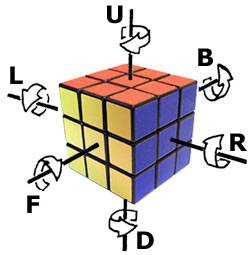
\includegraphics{img/giros}
  \caption{Movimientos posibles}
  \label{fig:ejemplo}
\end{figure}

El programa se probará con una herramienta que verifica que dada una receta y un cubo, ésta sea solución del mismo. Se correrá con miles de casos de prueba, por lo que el programa debe ser razonablemente rápido (10 segundos es mucho) y correcto en todos los casos. Teniendo en cuenta que el espacio de los cubos es enorme, esta cantidad de casos de prueba representa una pequeña fracción del total.


\section{Representación del problema}

Se puede pensar el problema de resolver el cubo de Rubik como una búsqueda en un espacio de estados, en donde se parte desde el cubo dado y se debe llegar mediante los movimientos de las caras al cubo resuelto. 


\subsection{Problemas de búsqueda}
El problema que queremos resolver se presta mucho a ser representado como un problema de búsqueda, por lo tanto comenzaremos por dar una noción básica de los mismos. \\
Típicamente, un problema de búsqueda se puede representar por 4 componentes:
\begin{itemize}
\item Un estado inicial
\item Un espacio de estados
\item Un conjunto de estados finales 
\item Varios operadores, que dado un estado, devuelven otro
\end{itemize}
En esencia, se puede pensar la búsqueda de una sucesión de operaciones que lleven del estado inicial a algún estado final como la exploración del árbol que resulta de tener como raiz al estado inicial y como nodos hijos los estados resultantes de aplicar sucesivamente todos los operadores. La búsqueda terminará cuando se llegue a algún estado final deseado.\\

Existen varios algoritmos de búsqueda distintos, que difieren entre si en la forma en que recorren dicho árbol.\\

A continuación veremos algunos algoritmos que nos ayudarán a resolver el problema del cubo.
\subsubsection{Breadth-first search (BFS)}
Esta búsqueda consiste en recorrer el árbol \emph{por niveles}. Esto quiere decir que ningún nodo del nivel $n$ será visitado antes que uno del nivel $n-1$.
Es un algoritmo \emph{completo}. Esto quiere decir que siempre encuentra una solución (si existe). También vemos que al encontrar una solución, ésta es ``óptima'', ya que no puede haber ningún otra solución en un nivel superior. \\

Para mantener este orden de los nodos, se debe implementar una cola, que contendrá los nodos todavia no \emph{expandidos}. \\

Sea $b$ la cantidad promedio de hijos por nodo. Si la solución está a una profundidad $d$, la complejidad temporal está en $O(b^d)$. La complejidad espacial también está en $O(b^d)$. \\  % como se justifica que la comp espacial esta en O(b^d)?

La figura \ref{fig:BFS} muestra el orden en el que se visitan los nodos para un árbol de ejemplo. \\

{
\begin{figure}[H]
  \centering
    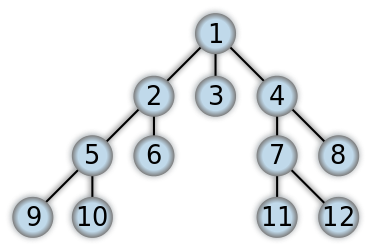
\includegraphics[width=0.7\textwidth]{img/BFS}
  \caption{Recorrido primero en anchura (BFS)}
  \label{fig:BFS}
\end{figure}
}
\subsubsection{Depth-first search (DFS)}
Esta búsqueda consiste en recorrer el árbol avanzando \emph{primero en profundidad}. Esto quiere decir que siempre que el nodo actual tenga hijos, se recorren estos, antes que los hermanos. \\

Este algoritmo también es completo (para un árbol finito), pero en general, no encuentra la solución óptima. La implementación es análoga al BFS, sólo que la estructura en donde se guardan los nodos pasa a ser una pila en vez de una cola. Gracias a esta, se implementa de una manera bastante directa con recursión, donde la pila de nodos queda implícita por la pila de llamadas a función. \\

La complejidad temporal está en $O(b^{d})$, donde $d$ es la máxima profundidad del árbol. La complejidad espacial es bastante razonable: $O(d)$. \\

La figura \ref{fig:DFS} muestra el orden en el que se visitan los nodos para un árbol de ejemplo.

{
\begin{figure}[]
  \centering
    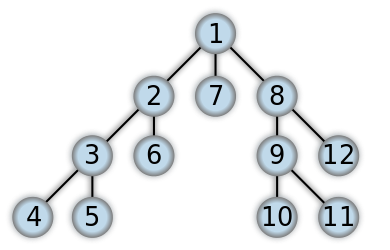
\includegraphics[width=0.7\textwidth]{img/DFS}
  \caption{Recorrido primero en profundidad (DFS)}
  \label{fig:DFS}
\end{figure}
}

\subsubsection{DFS con Profundidad Acotada}
Consiste en utilizar la búsqueda DFS con una cota $l$ en la profundidad, de manera tal que los nodos del nivel $l+1$ en adelante sean ignorados. 
\begin{itemize}
\item ¿Es completa esta búsqueda? ¿Bajo que condiciones?.
\item ¿Es óptima esta búsqueda? ¿Bajo que condiciones?.
\item ¿Cuales son sus complejidades espaciales y temporales?.
\item Supongamos que un DFS con profundidad acotada $n$ no encuentra solución, pero un DFS con profundidad acotada $n+1$ si encuentra. ¿Que se puede concluir respecto a la solución? 
\item Usando la idea del ítem anterior, ¿puede diseñar una búsqueda completa y óptima basada en el DFS?
\end{itemize}

\section{Más sobre búsqueda}
Hay varios temas a considerar al programar un algoritmo de búsqueda. Primero y principal, la elección de un algoritmo adecuado según la búsqueda que necesitemos hacer. Pensemos en un cubo de Rubik que necesita 20 pasos para resolverse. Partimos de ese estado inicial y buscamos una receta que solucione el cubo. \\

Si elegimos una búsqueda óptima, se expandirán todos los nodos a distancia 19 del original, ya que no hay una receta de longitud 19 o menor que lo resuelva\footnotemark. La cantidad de nodos en el nivel 19 es un número en el orden de $11^{19}$, un número inmensamente grande. Una búsqueda con estas características no terminaría en tiempo razonable, por lo que no podríamos implementarlo de esta manera. Algunas ideas para mejorar esto son:

\footnotetext{Si es alguna búsqueda que expanda todos los nodos del nivel $n$ antes del $n+1$, como el BFS. Hay otras búsquedas que usando \emph{heurísticas}, pueden garantizar la optimalidad de la solución sin esta desventaja.}

\begin{itemize}
\item \textbf{No buscar una solución óptima.} Debilitar los requerimientos puede facilitar la tarea. 
\item \textbf{Dividir la búsqueda en etapas.} Podemos hacer búsquedas parciales para ir resolviendo el cubo, usando una búsqueda (óptima o no) entre etapas. Notar que la optimalidad de las receta parciales no garantiza la optimalidad de la receta final.
Con una buena elección de las etapas, la complejidad (tanto espacial como temporal) disminuye mucho.
\item \textbf{Usar una heurística.} Una heurística es una función que estima la distancia de un nodo (cubo) hasta la meta (cubo resuelto). Usando estas funciones podemos usar métodos de búsqueda \emph{con información}, que dan mejores resultados respecto a cantidad de nodos expandidos.
\item \textbf{Aprovechar conocimiento específico del dominio.} % Bueeeena ING SOFT
No es necesario que nuestro método de búsqueda sea general y sirva para cualquier problema. Queremos un programa que solamente resuelva el cubo de Rubik, entonces podemos aprovechar información específica sobre el cubo de Rubik que puede no aplicar a otros problemas.
\end{itemize}

%\subsubsection{DFS con Profunidad Iterativa}
%Consiste en utilizar reiteradas veces el algoritmo anterior, comenzando con $l \; = \; 0$ y aumentando $l$ en 1 por cada iteración.
%De esta forma, tomando como referencia le figura correspondiente al DFS, en cada iteración los nodos recorridos serán los siguientes: 
%\begin{itemize}
%\item 1
%\item 1, 2, 7, 8
%\item 1, 2, 3, 6, 7, 8, 9, 12 
%\item 1, 2, 3, 4, 5, 6, 7, 8, 9, 10, 11, 12
%\end{itemize}  

% falta poner bibliografia 







\begin{thebibliography}{9}

\bibitem{movs}
  http://www.cube20.org/
  
\end{thebibliography}

\end{document}
